\documentclass[11pt]{article}
\usepackage[margin=1in]{geometry}
\usepackage[T1]{fontenc}
\usepackage{listings}
\lstset{basicstyle=\ttfamily\footnotesize,frame=single,breaklines=true,columns=fullflexible,keepspaces=true}
\usepackage{booktabs}
\usepackage{float}
\usepackage{array}
\usepackage{pgfplots}
\usetikzlibrary{arrows.meta,decorations.pathreplacing,calc,shapes.geometric}
\usepgfplotslibrary{groupplots,fillbetween}
\pgfplotsset{compat=1.18}
\usepackage{hyperref}
\usepackage{xurl}
\emergencystretch=3em

\title{Custom UDP Server vs.\ Godot ENet:\\[0.5ex]A Cloud Benchmark of Multiplayer Server Capacity}
\author{Carlos Nunez\\
Department of Computer Science and Engineering, Shippensburg University\\
Mentor: Dr.\ Girard\\
CSC 499 -- Senior Research Methods}
\date{Fall 2026 (draft)}

\begin{document}
\maketitle

\begin{abstract}
Developers who build multiplayer games in Godot must choose between the engine's built-in
ENet dedicated server and a custom server written outside the engine. We compare a custom C++ UDP
server with Godot's ENet headless server under the same workload, NodeStrike, a 20×20 grid game
in which every client is a bot that moves one tile per 20~Hz server tick. Both servers run on
Google Cloud with one server VM and three client VMs. Two tests are used: a progressive
ladder that adds clients from 1 to 300, run eight times per backend, and a 20-minute hold at fixed loads of 180 to 300
clients. We measure latency, packet handling (snapshots received per client per second), client limit, and server
tick rate. Across the eight ladder runs the C++ server passed all 292 states every time, with a round-trip time near 6~ms.
ENet passed at 100 and 150 clients in all eight runs, at 200 clients in three of eight, and at 250 clients in none; its first
failure came between 170 and 188 clients in every run, with ping and lost snapshots growing beyond that. In the 20-minute
holds, C++ kept every client responding at 180, 260, 270 and 300 clients in all eight runs, with ping near 6~ms. ENet held 180 clients in all
eight runs, but held 260 and 270 clients in only one run each and 300 clients in none; at 300 clients about 75\% of its clients responded and
ping was near 1.4~s. ENet's server tick rate stayed near 20~Hz throughout, so tick rate alone did not reveal its overload.
Both tests are the mean of eight complete runs per backend.
\end{abstract}

\noindent\textbf{Keywords:} game networking, UDP, ENet, Godot, tick rate, server capacity, benchmarking

\section{Introduction}
TODO: write the introduction (problem, what this paper does, the questions).

\section{Background and Related Work}
TODO: write the background (servers and transport, related work).

\subsection{Ticks and snapshots}
TODO: write what a tick and a snapshot are.

\begin{table}[H]
\centering
\small
\begin{tabular}{@{}p{0.2\textwidth}p{0.72\textwidth}@{}}
\toprule
Term & Meaning in NodeStrike \\
\midrule
Hz (hertz) & Times per second. NodeStrike runs at 20~Hz, i.e.\ 20 ticks per second. \\
Tick & One server cycle: read incoming client updates, update the world, send a snapshot. Fixed at 50~ms ($1000/20$). \\
Snapshot & A capture of the game state at one tick: every player's position at that instant. The server sends it to each client ($16 + 12N$ bytes for $N$ players, split into datagrams of at most 1{,}200 bytes). Each arrival updates the client's current ping reading and gap count. \\
Latency / ping & How long data takes to travel. Round-trip time (RTT) is there and back. In the game client, ping is the time from sending its last position update until the next snapshot arrives, so it includes waiting for the server's next 50~ms tick. \\
Gap / loss & Each snapshot has a sequence number; a missing number means a snapshot was lost or dropped. \\
Effective tick rate & Ticks the server actually completes per second. Healthy $\approx 20$~Hz; below 18~Hz is treated as overloaded. \\
\bottomrule
\end{tabular}
\caption{Terms used in this paper.}\label{tab:terms}
\end{table}

\begin{figure}[H]
\centering
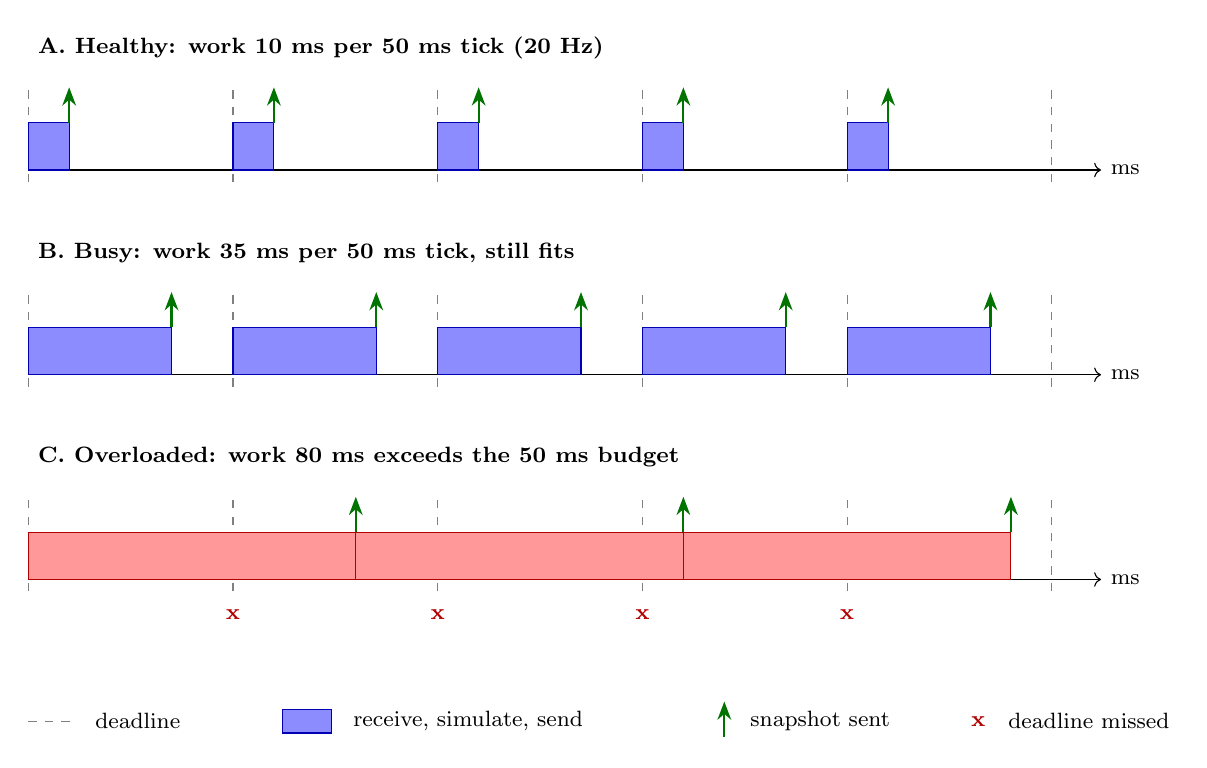
\begin{tikzpicture}[x=0.052cm,y=1cm,font=\footnotesize]
\tikzset{work/.style={fill=blue!45,draw=blue!70!black},
         late/.style={fill=red!40,draw=red!70!black},
         snap/.style={-{Stealth},thick,green!45!black},
         dl/.style={dashed,gray}}

\begin{scope}[yshift=0cm]
\node[anchor=west] at (0,1.55) {\textbf{A. Healthy: work 10 ms per 50 ms tick (20 Hz)}};
\foreach \t in {0,50,...,250} {\draw[dl] (\t,-0.15) -- (\t,1.1);}
\draw[->] (0,0) -- (262,0) node[right]{ms};
\foreach \t in {0,50,100,150,200} {
  \filldraw[work] (\t,0) rectangle (\t+10,0.6);
  \draw[snap] (\t+10,0.6) -- (\t+10,1.05);}
\end{scope}

\begin{scope}[yshift=-2.6cm]
\node[anchor=west] at (0,1.55) {\textbf{B. Busy: work 35 ms per 50 ms tick, still fits}};
\foreach \t in {0,50,...,250} {\draw[dl] (\t,-0.15) -- (\t,1.1);}
\draw[->] (0,0) -- (262,0) node[right]{ms};
\foreach \t in {0,50,100,150,200} {
  \filldraw[work] (\t,0) rectangle (\t+35,0.6);
  \draw[snap] (\t+35,0.6) -- (\t+35,1.05);}
\end{scope}

\begin{scope}[yshift=-5.2cm]
\node[anchor=west] at (0,1.55) {\textbf{C. Overloaded: work 80 ms exceeds the 50 ms budget}};
\foreach \t in {0,50,...,250} {\draw[dl] (\t,-0.15) -- (\t,1.1);}
\draw[->] (0,0) -- (262,0) node[right]{ms};
\foreach \t in {0,80,160} {
  \filldraw[late] (\t,0) rectangle (\t+80,0.6);
  \draw[snap] (\t+80,0.6) -- (\t+80,1.05);}
\foreach \t in {50,100,150,200} {\node[red!70!black] at (\t,-0.45) {\textbf{x}};}
\end{scope}

\begin{scope}[yshift=-7.2cm]
\draw[dl] (0,0.2) -- (12,0.2); \node[anchor=west] at (14,0.2) {deadline};
\filldraw[work] (62,0.05) rectangle (74,0.35); \node[anchor=west] at (77,0.2) {receive, simulate, send};
\draw[snap] (170,0.0) -- (170,0.45); \node[anchor=west] at (174,0.2) {snapshot sent};
\node[red!70!black] at (232,0.2) {\textbf{x}}; \node[anchor=west] at (237,0.2) {deadline missed};
\end{scope}
\end{tikzpicture}
\caption{Schematic of a server tick (illustrative timings, not measured data).
Each tick the server receives client input, updates the world, and sends a
snapshot; at 20~Hz it has 50~ms for all of it. If the work per tick grows with
the number of clients and passes 50~ms, ticks start late, the effective tick rate
falls ($1000/80=12.5$~Hz in panel~C) and clients get fewer, later snapshots.}
\label{fig:tickvisual}
\end{figure}

\section{Making of the Godot Client and ENet Server}
TODO: write how the Godot client and the Godot ENet server were built (goals, design decisions, problems you hit).

\paragraph{Notes from the code (delete when written).}
\begin{itemize}
\item One Godot 4.7 project, NodeStrike (20×20 grid). One script, \texttt{main.gd} (about 860 lines), runs every role.
\item The role is chosen with command-line flags: \texttt{--transport=udp|enet}, \texttt{--role=client|server}, \texttt{--address}, \texttt{--port}, \texttt{--udp-only}, \texttt{--enet-snapshot=binary|variant}.
\item Client: spawns a bot, picks a goal tile, moves one tile per tick from a 20~Hz timer, and sends its position every tick (an 18-byte message over UDP, or a remote procedure call over ENet).
\item Client default is the C++ UDP server; a windowed client falls back to ENet after 8~s with no reply, unless \texttt{--udp-only} is set.
\item ENet server mode: creates an ENet multiplayer peer (up to 2048 clients), runs a 20~Hz timer, drops clients silent for more than 5~s, and each tick sends one snapshot to every peer by remote procedure call (compact binary, or a list of dictionaries).
\item Headless mode (no window) is used for the benchmark and prints ping, packets sent and received, and gaps in snapshot numbers.
\item Two small extra scripts, \texttt{enet\_server.gd} and \texttt{enet\_client.gd}, are a simpler ENet pair that the cloud benchmark does not use.
\end{itemize}

\begin{figure}[H]
\centering
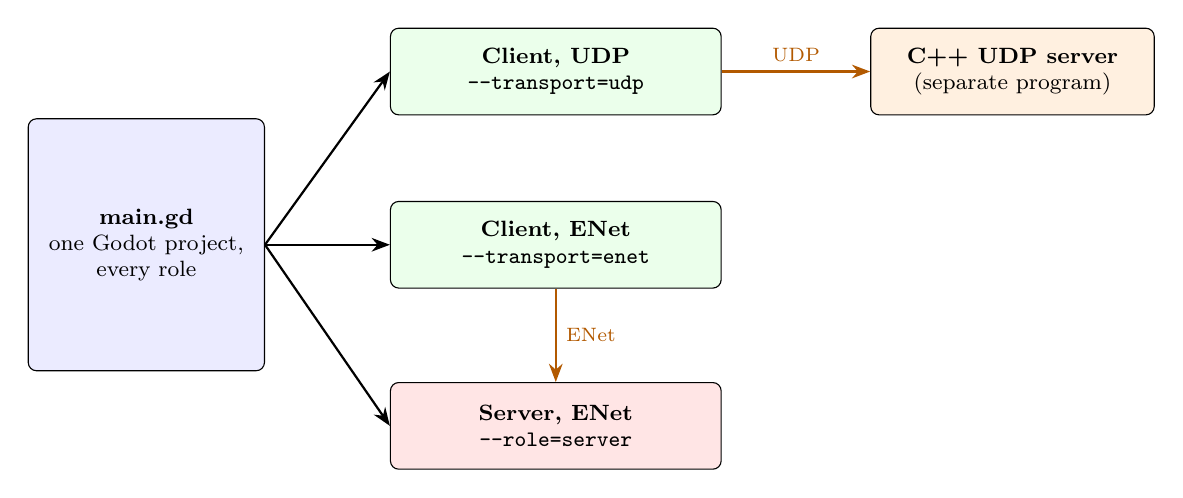
\begin{tikzpicture}[x=1cm,y=1cm,font=\footnotesize,
  box/.style={draw,rounded corners=3pt,align=center,inner sep=5pt,minimum height=1.1cm},
  arr/.style={-{Stealth},thick}]
\node[box,fill=blue!8,minimum width=3.0cm,minimum height=3.2cm] (main) at (0,0) {\textbf{main.gd}\\ one Godot project,\\ every role};
\node[box,fill=green!8,minimum width=4.2cm] (m1) at (5.2,2.2) {\textbf{Client, UDP}\\ \texttt{--transport=udp}};
\node[box,fill=green!8,minimum width=4.2cm] (m2) at (5.2,0) {\textbf{Client, ENet}\\ \texttt{--transport=enet}};
\node[box,fill=red!10,minimum width=4.2cm] (m3) at (5.2,-2.3) {\textbf{Server, ENet}\\ \texttt{--role=server}};
\node[box,fill=orange!12,minimum width=3.6cm] (cpp) at (11,2.2) {\textbf{C++ UDP server}\\ (separate program)};
\foreach \m in {m1,m2,m3} {\draw[arr] (main.east) -- (\m.west);}
\draw[arr,orange!70!black] (m1.east) -- (cpp.west) node[midway,above,font=\scriptsize] {UDP};
\draw[arr,orange!70!black] (m2.south) -- (m3.north) node[midway,right,font=\scriptsize] {ENet};
\end{tikzpicture}
\caption{The Godot project. One script is started in different modes. A UDP client talks to the separate C++ server; an ENet client talks to the same project started as an ENet server.}
\end{figure}

\section{Making of the C++ UDP Server}
TODO: write how the C++ server was built (goals, design decisions, problems you hit).

\paragraph{Notes from the code (delete when written).}
\begin{itemize}
\item One file, \texttt{server/main.cpp} (about 590 lines), C++17, plain POSIX sockets, one thread.
\item Binary protocol, version 2 (Table~\ref{tab:packets}). A player is identified by its network address, not by anything the client sends.
\item Main loop (Figure~\ref{fig:cppLoop}): wait up to 5~ms for a packet, read everything waiting, and when 50~ms have passed since the last tick, run a tick.
\item A tick drops clients silent for more than 5~s and sends a snapshot to every client, split into datagrams of at most 1,200 bytes.
\item Once a second it prints one telemetry line (tick number, players, packets and bytes in and out); the benchmark records these lines.
\item A separate terminal display, \texttt{tui/tui.cpp}, exists for watching a server.
\end{itemize}

\begin{table}[H]
\centering
\small
\begin{tabular}{@{}llrl@{}}
\toprule
Message & Direction & Size & Contents \\
\midrule
JOIN & client to server & 2 B & type, version \\
ACK & server to client & 6 B & type, version, player id \\
STATE & client to server & 18 B & position, timestamp, number, goal \\
PING & both ways & 10 B & client timestamp, number (echoed back) \\
TICK (snapshot) & server to client & 16 + 12N B & header, then id, position and goal for each of N players \\
\bottomrule
\end{tabular}
\caption{Messages of the C++ server protocol (version 2). Snapshots larger than 1,200 bytes are split into several datagrams.}
\label{tab:packets}
\end{table}

\begin{figure}[H]
\centering
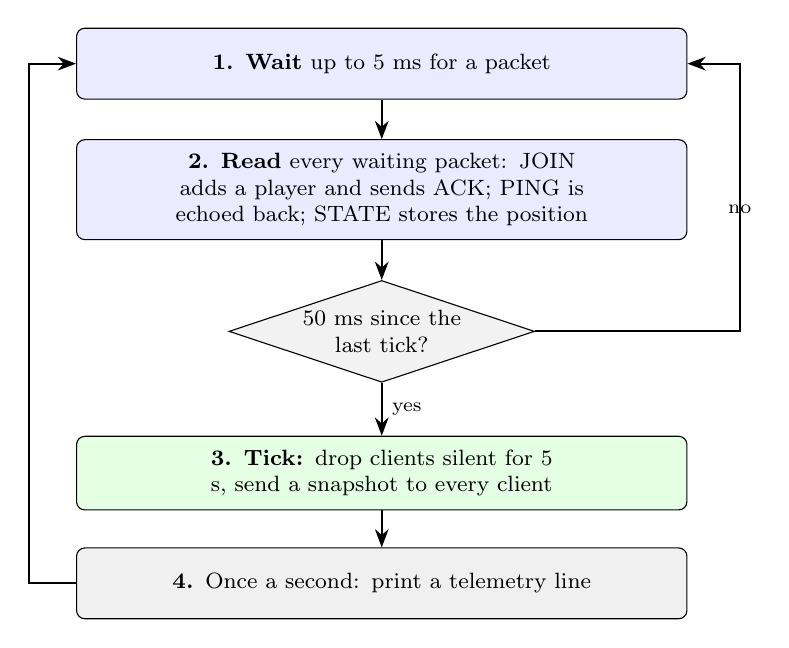
\begin{tikzpicture}[x=1cm,y=1cm,font=\footnotesize,
  box/.style={draw,rounded corners=3pt,align=center,inner sep=5pt,text width=7.4cm,minimum height=0.9cm},
  dec/.style={draw,diamond,aspect=3,align=center,inner sep=1pt,fill=gray!10},
  arr/.style={-{Stealth},thick}]
\node[box,fill=blue!8] (a) at (0,0) {\textbf{1. Wait} up to 5 ms for a packet};
\node[box,fill=blue!8] (b) at (0,-1.6) {\textbf{2. Read} every waiting packet: JOIN adds a player and sends ACK; PING is echoed back; STATE stores the position};
\node[dec] (c) at (0,-3.4) {50 ms since the\\ last tick?};
\node[box,fill=green!10] (d) at (0,-5.2) {\textbf{3. Tick:} drop clients silent for 5 s, send a snapshot to every client};
\node[box,fill=gray!12] (e) at (0,-6.6) {\textbf{4.} Once a second: print a telemetry line};
\draw[arr] (a) -- (b);
\draw[arr] (b) -- (c);
\draw[arr] (c) -- (d) node[midway,right,font=\scriptsize] {yes};
\draw[arr] (d) -- (e);
\draw[arr] (c.east) -- ++(2.6,0) |- (a.east) node[pos=0.2,above,font=\scriptsize] {no};
\draw[arr] (e.west) -- ++(-0.6,0) |- (a.west);
\end{tikzpicture}
\caption{Main loop of the C++ server. It repeats forever on one thread.}
\label{fig:cppLoop}
\end{figure}

\section{How Both Servers Work: The Ins and Outs}
TODO: write how the two servers work and how they differ.

\begin{table}[H]
\centering
\small
\begin{tabular}{@{}p{0.2\textwidth}p{0.36\textwidth}p{0.36\textwidth}@{}}
\toprule
& C++ UDP server & Godot ENet server \\
\midrule
Networking & raw UDP datagrams & ENet through Godot's multiplayer peer \\
Default port & 7777 & 7778 \\
Tick timing & polls the clock every few ms and restarts its timer after each tick (about 19 ticks per second) & Godot timer that fires every 50 ms (about 20 ticks per second) \\
Join & JOIN message, ACK with player id & connection handled by ENet; the peer id is the player id \\
Position update & 18-byte STATE datagram & remote procedure call (unreliable) \\
Snapshot & 16 + 12N bytes, split into datagrams of at most 1,200 B & 8 + 12N bytes (binary format), one remote procedure call \\
Client eviction & silent for 5 s & silent for 5 s \\
Latency measure & dedicated PING message echoed by the server & game client's ping: last send until next snapshot \\
Telemetry & one line per second & periodic server statistics \\
\bottomrule
\end{tabular}
\caption{The two backends side by side.}
\label{tab:compare}
\end{table}

\begin{figure}[H]
\centering
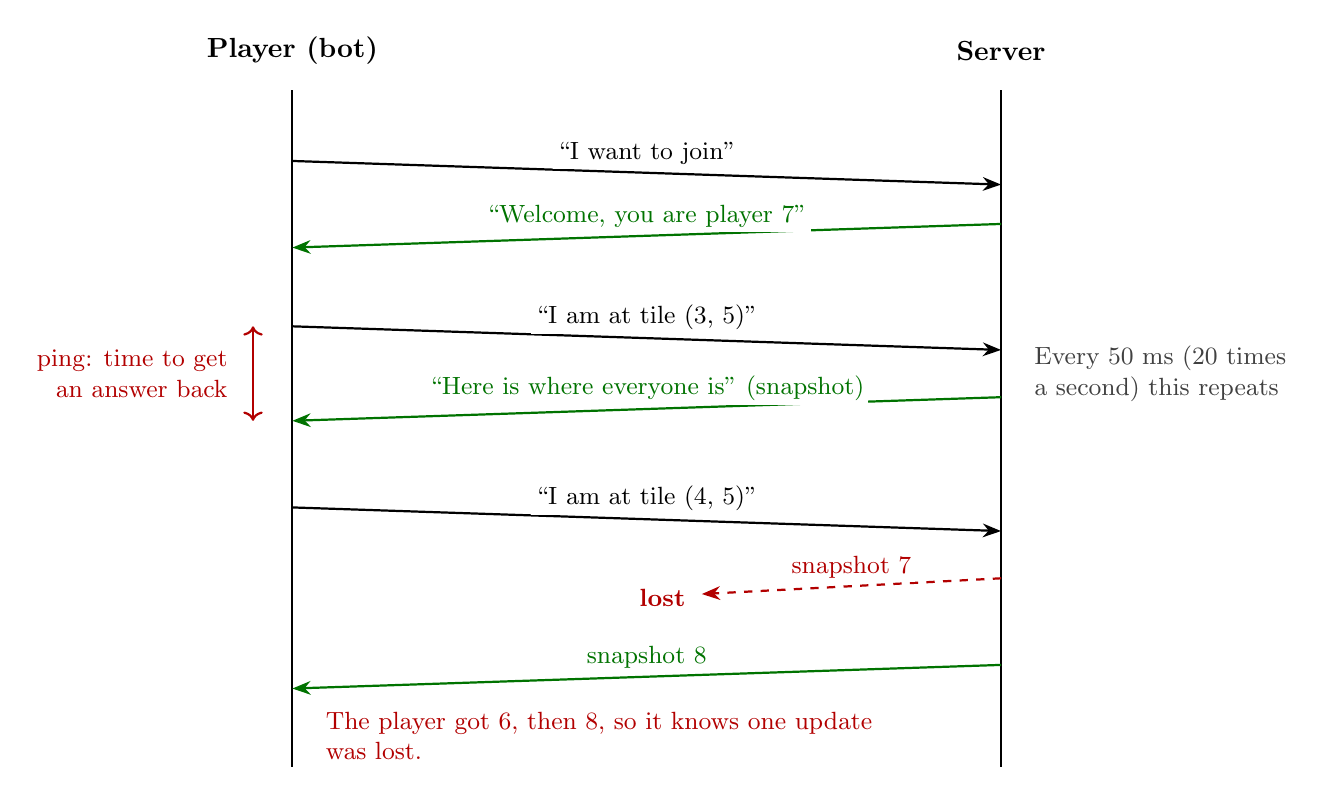
\begin{tikzpicture}[x=1cm,y=1cm,font=\small]
\tikzset{msg/.style={-{Stealth},thick},
         note/.style={fill=white,inner sep=1.5pt}}
\node[font=\bfseries\normalsize] at (0,0.5) {Player (bot)};
\node[font=\bfseries\normalsize] at (9,0.5) {Server};
\draw[thick] (0,0) -- (0,-8.6);
\draw[thick] (9,0) -- (9,-8.6);

% 1 join
\draw[msg] (0,-0.9) -- (9,-1.2) node[midway,note,above=1pt] {``I want to join''};
\draw[msg,green!45!black] (9,-1.7) -- (0,-2.0) node[midway,note,above=1pt] {``Welcome, you are player 7''};

% 2 normal round
\node[anchor=west,text width=3.2cm,align=left,gray!50!black] at (9.3,-3.6) {Every 50 ms (20 times a second) this repeats};
\draw[msg] (0,-3.0) -- (9,-3.3) node[midway,note,above=1pt] {``I am at tile (3, 5)''};
\draw[msg,green!45!black] (9,-3.9) -- (0,-4.2) node[midway,note,above=1pt] {``Here is where everyone is'' (snapshot)};
\draw[<->,red!70!black,thick] (-0.5,-3.0) -- (-0.5,-4.2);
\node[red!70!black,anchor=east,align=right] at (-0.7,-3.6) {ping: time to get\\ an answer back};

% 3 lost
\draw[msg] (0,-5.3) -- (9,-5.6) node[midway,note,above=1pt] {``I am at tile (4, 5)''};
\draw[msg,red!70!black,dashed] (9,-6.2) -- (5.2,-6.4) node[midway,note,above=1pt,text=red!70!black] {snapshot 7};
\node[red!70!black,font=\bfseries\small] at (4.7,-6.45) {lost};
\draw[msg,green!45!black] (9,-7.3) -- (0,-7.6) node[midway,note,above=1pt] {snapshot 8};
\node[anchor=west,text width=7.5cm,red!70!black] at (0.3,-8.2) {The player got 6, then 8, so it knows one update was lost.};
\end{tikzpicture}
\caption{What the player and the server say to each other. The player says where
it is, the server replies with where everyone is, and this repeats 20 times a
second. Ping is how long it takes to hear back; a lost reply shows up as a missing
number. The ENet backend does the same thing through Godot's own networking.}
\label{fig:flow}
\end{figure}

\subsection{One tick, step by step}
Every 50~ms the server does the same five things, in this order. If steps 1 to 4
take less than 50~ms, it waits for the next tick. If they take longer, the next
tick starts late.

\begin{figure}[!htbp]
\centering
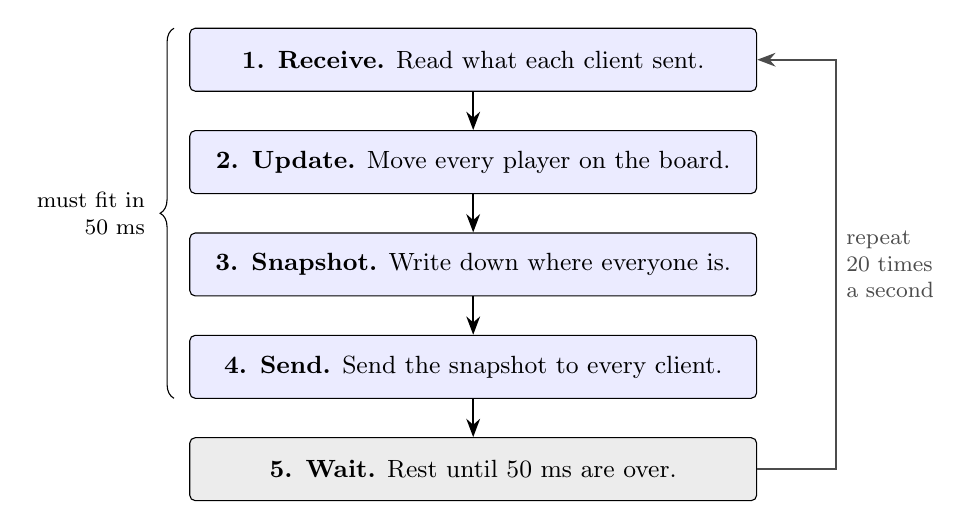
\begin{tikzpicture}[x=1cm,y=1cm,font=\small,
  stepbox/.style={draw,rounded corners=2pt,fill=blue!8,minimum width=7.2cm,minimum height=0.8cm,align=left,inner sep=5pt},
  waitbox/.style={draw,rounded corners=2pt,fill=gray!15,minimum width=7.2cm,minimum height=0.8cm,align=left,inner sep=5pt},
  down/.style={-{Stealth},thick}]
\node[stepbox] (a) at (0,0) {\textbf{1. Receive.} Read what each client sent.};
\node[stepbox] (b) at (0,-1.3) {\textbf{2. Update.} Move every player on the board.};
\node[stepbox] (c) at (0,-2.6) {\textbf{3. Snapshot.} Write down where everyone is.};
\node[stepbox] (d) at (0,-3.9) {\textbf{4. Send.} Send the snapshot to every client.};
\node[waitbox] (e) at (0,-5.2) {\textbf{5. Wait.} Rest until 50 ms are over.};
\foreach \p/\q in {a/b,b/c,c/d,d/e} {\draw[down] (\p.south) -- (\q.north);}
\draw[down,gray!60!black] (e.east) -- ++(1.0,0) |- (a.east) node[pos=0.25,right,align=left,font=\footnotesize] {repeat\\ 20 times\\ a second};
\draw[decorate,decoration={brace,amplitude=5pt,mirror}] (-3.8,0.4) -- (-3.8,-4.3) node[midway,left=7pt,align=right,font=\footnotesize] {must fit in\\ 50 ms};
\end{tikzpicture}
\caption{The server tick. Steps 1 to 4 are the work; step 5 is spare time. The
more clients there are, the longer steps 3 and 4 take.}
\end{figure}

\subsection{Why more clients means much more work}
Each snapshot lists every player, and every client gets one. So when the number of
clients $N$ doubles, each snapshot gets about twice as big and there are twice as
many to send: the work grows about four times. Figure~\ref{fig:growth} shows the
amount of data this means for the C++ server (snapshot of $16 + 12N$ bytes sent to
$N$ clients, 20 times a second).

\begin{figure}[!htbp]
\centering
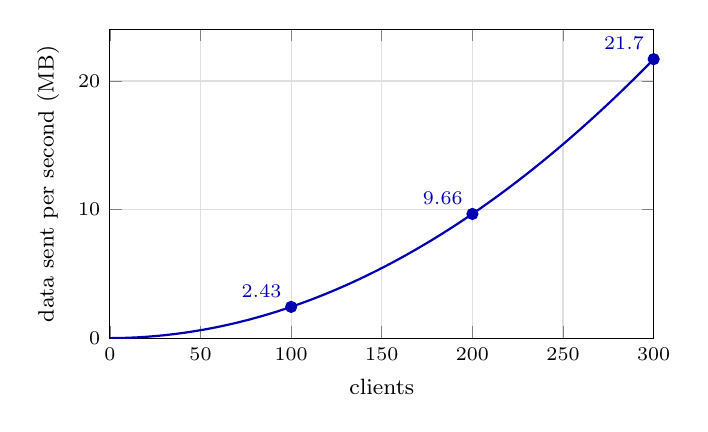
\begin{tikzpicture}
\begin{axis}[width=0.7\textwidth,height=5.5cm,xlabel={clients},ylabel={data sent per second (MB)},
  xmin=0,xmax=300,ymin=0,ymax=24,grid=major,grid style={gray!25},
  tick label style={font=\scriptsize},label style={font=\footnotesize}]
\addplot[blue!70!black,thick,domain=0:300,samples=60]{20*x*(16+12*x)/1000000};
\addplot[only marks,mark=*,mark size=2pt,blue!70!black,nodes near coords,
  every node near coord/.append style={font=\scriptsize,anchor=south east}]
  coordinates {(100,2.43) (200,9.66) (300,21.7)};
\end{axis}
\end{tikzpicture}
\caption{Data the server must send each second as clients are added (calculated
from the packet format; ENet is similar). Tripling the clients from 100 to 300
multiplies the data about nine times.}
\label{fig:growth}
\end{figure}

\subsection{How clients end up responding less (and recovering)}\label{sec:chain}
A client counts as \textit{responding} if it received at least one new snapshot during the
measurement period. While the server keeps up, every client gets a snapshot every
tick. Once the work per tick is too much, snapshots arrive late, get skipped, or
pile up behind each other, and some clients stop receiving any. Figure~\ref{fig:chain}
shows the chain of events, and Figure~\ref{fig:arrivals} shows what one client sees.

\begin{figure}[!htbp]
\centering
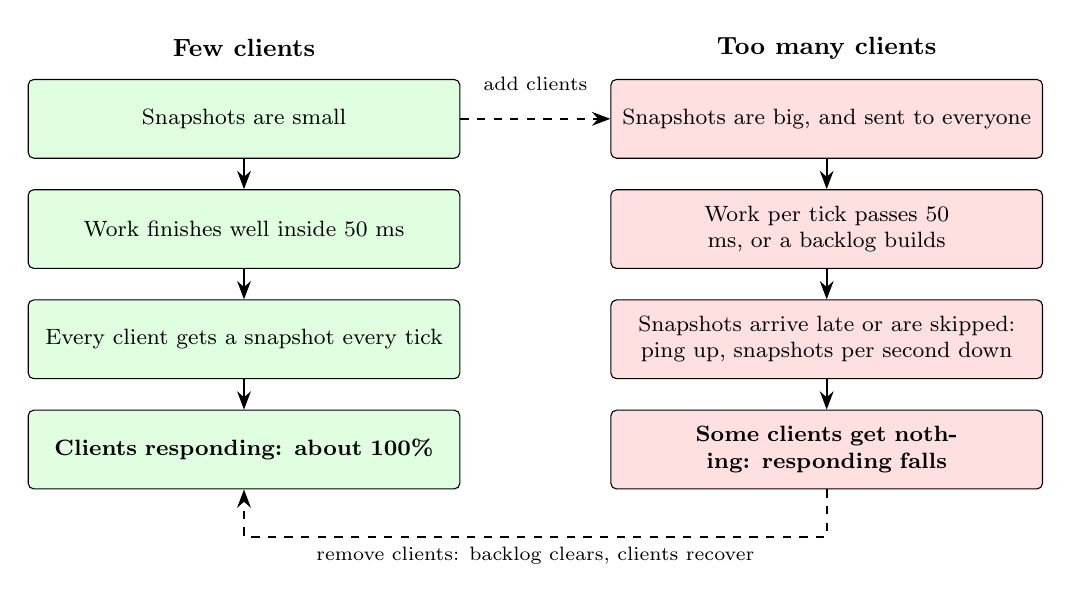
\begin{tikzpicture}[x=1cm,y=1cm,font=\footnotesize,
  box/.style={draw,rounded corners=2pt,text width=5.2cm,minimum height=1.0cm,align=center,inner sep=4pt},
  good/.style={box,fill=green!12},bad/.style={box,fill=red!12},
  down/.style={-{Stealth},thick}]
\node[font=\bfseries\small] at (-3.6,0.9) {Few clients};
\node[font=\bfseries\small] at (3.8,0.9) {Too many clients};
\node[good] (g1) at (-3.6,0) {Snapshots are small};
\node[good] (g2) at (-3.6,-1.4) {Work finishes well inside 50 ms};
\node[good] (g3) at (-3.6,-2.8) {Every client gets a snapshot every tick};
\node[good] (g4) at (-3.6,-4.2) {\textbf{Clients responding: about 100\%}};
\node[bad] (b1) at (3.8,0) {Snapshots are big, and sent to everyone};
\node[bad] (b2) at (3.8,-1.4) {Work per tick passes 50 ms, or a backlog builds};
\node[bad] (b3) at (3.8,-2.8) {Snapshots arrive late or are skipped: ping up, snapshots per second down};
\node[bad] (b4) at (3.8,-4.2) {\textbf{Some clients get nothing: responding falls}};
\foreach \p/\q in {g1/g2,g2/g3,g3/g4,b1/b2,b2/b3,b3/b4} {\draw[down] (\p) -- (\q);}
\draw[-{Stealth},thick,dashed] (g1.east) -- (b1.west);
\node[font=\scriptsize] at (0.1,0.45) {add clients};
\draw[-{Stealth},thick,dashed] (b4.south) -- ++(0,-0.6) -| (g4.south) node[pos=0.25,below,font=\scriptsize] {remove clients: backlog clears, clients recover};
\end{tikzpicture}
\caption{Left: a server that keeps up. Right: how adding clients leads to fewer
clients responding. The dashed arrows show that removing load reverses it.}
\label{fig:chain}
\end{figure}

\begin{figure}[!htbp]
\centering
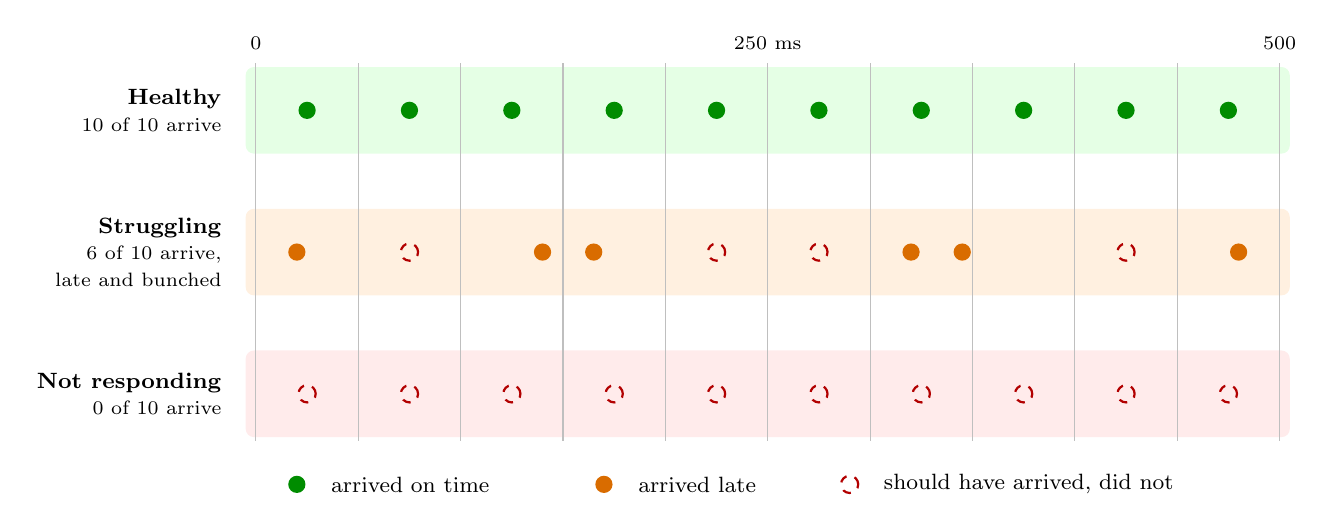
\begin{tikzpicture}[x=0.026cm,y=1cm,font=\footnotesize,
  got/.style={circle,fill=green!55!black,inner sep=2.2pt},
  late/.style={circle,fill=orange!85!black,inner sep=2.2pt},
  miss/.style={circle,draw=red!70!black,dashed,thick,inner sep=2.2pt}]
\fill[green!10,rounded corners=3pt] (-5,-0.55) rectangle (505,0.55);
\fill[orange!12,rounded corners=3pt] (-5,-2.35) rectangle (505,-1.25);
\fill[red!8,rounded corners=3pt] (-5,-4.15) rectangle (505,-3.05);
\foreach \t in {0,50,...,500} {\draw[gray!50,thin] (\t,0.6) -- (\t,-4.2);}
\node[anchor=south,font=\scriptsize] at (0,0.65) {0};
\node[anchor=south,font=\scriptsize] at (250,0.65) {250 ms};
\node[anchor=south,font=\scriptsize] at (500,0.65) {500};
\node[anchor=east,align=right] at (-12,0) {\textbf{Healthy}\\ \scriptsize 10 of 10 arrive};
\node[anchor=east,align=right] at (-12,-1.8) {\textbf{Struggling}\\ \scriptsize 6 of 10 arrive,\\ \scriptsize late and bunched};
\node[anchor=east,align=right] at (-12,-3.6) {\textbf{Not responding}\\ \scriptsize 0 of 10 arrive};
\foreach \t in {25,75,...,475} {\node[got] at (\t,0) {};}
\foreach \t in {20,140,165,320,345,480} {\node[late] at (\t,-1.8) {};}
\foreach \t in {75,225,275,425} {\node[miss] at (\t,-1.8) {};}
\foreach \t in {25,75,...,475} {\node[miss] at (\t,-3.6) {};}
\node[got] at (20,-4.75) {}; \node[anchor=west] at (32,-4.75) {arrived on time};
\node[late] at (170,-4.75) {}; \node[anchor=west] at (182,-4.75) {arrived late};
\node[miss] at (290,-4.75) {}; \node[anchor=west] at (302,-4.75) {should have arrived, did not};
\end{tikzpicture}
\caption{What one client receives over 500~ms (schematic). Each dot is a snapshot
the server should send every 50~ms. Healthy: all arrive on time. Struggling: some
come late and bunched together, others never arrive. Not responding: none arrive,
so the client is counted as not responding.}
\label{fig:arrivals}
\end{figure}

\section{Experimental Method}\label{sec:data}

All runs use one server VM and three client VMs on Google Cloud (e2-standard-2 machines).
ENet snapshots use the binary format from 22 September onward.

\subsection{Main measures}
Three measures are the main focus of the study. The rest of the data (CPU, memory,
network use, server counters and every other column collected) is kept and still matters:
it is used to explain why the main measures change. A tick-rate drop is the warning sign
that one of the three is failing.

\begin{table}[H]
\centering
\small
\begin{tabular}{@{}p{0.2\textwidth}p{0.36\textwidth}p{0.31\textwidth}@{}}
\toprule
Measure & Plain meaning & On the charts \\
\midrule
Latency & How long data takes to go to the server and back, in milliseconds (ping). Lower is better. & Ping in milliseconds (log scale) \\
Packet handling & How many packets the server receives and sends each second without losing or delaying them. A healthy client gets one snapshot per tick, about 20 per second. & Snapshots received per client per second (20 is perfect) \\
Client limit & The largest number of clients the server supports before performance degrades. & Share of clients still responding; where the lines break \\
Tick rate (warning sign) & Ticks the server completes per second. 20 Hz is healthy; below 18 Hz means the server is falling behind. & Server ticks per second, with an 18~Hz line \\
\bottomrule
\end{tabular}
\caption{The three main measures, and the tick-rate warning sign. All other collected data supports them.}
\end{table}


\subsection{Two kinds of test}
We run two kinds of test, because they answer different questions.

\begin{itemize}
\item \textbf{Progressive (granular) ladder.} Start with one client and add
clients one step at a time, holding each step for a short time (10~s in the
October runs). The state list is 1 client, then 10, 11, 12, up to 300: 292
states per backend. Question: at what client count does the server stop
keeping up?
\item \textbf{Hold.} Ramp up to a target client count (targets 180, 260,
270 and 300), stop adding clients, and keep them connected for 20 minutes,
measured in 120 windows of 10~s. Question: does the server stay stable at a
fixed load?
\end{itemize}

\begin{figure}[!htbp]
\centering
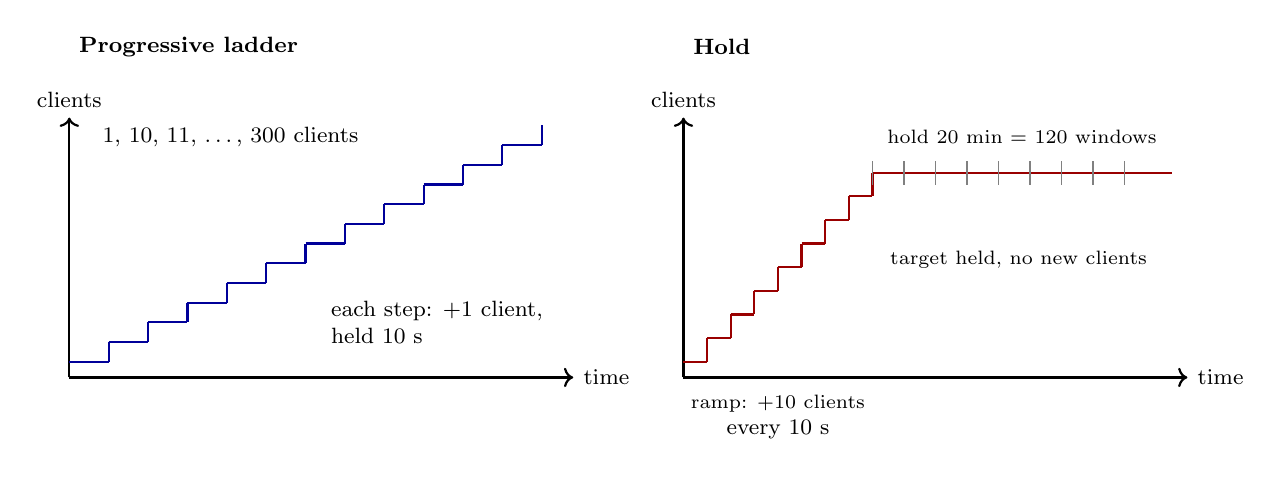
\begin{tikzpicture}[x=1cm,y=1cm,font=\footnotesize]
\tikzset{ax/.style={->,thick}}
\begin{scope}
\node[anchor=west,font=\bfseries\footnotesize] at (0,4.2) {Progressive ladder};
\draw[ax] (0,0) -- (6.4,0) node[right]{time};
\draw[ax] (0,0) -- (0,3.3) node[above]{clients};
\foreach \i in {0,...,11} {
  \draw[blue!60!black,thick] (\i*0.5,0.2+\i*0.25) -- (\i*0.5+0.5,0.2+\i*0.25);
  \draw[blue!60!black,thick] (\i*0.5+0.5,0.2+\i*0.25) -- (\i*0.5+0.5,0.45+\i*0.25);}
\node[anchor=west] at (0.3,3.05) {1, 10, 11, \dots, 300 clients};
\node[anchor=west,align=left] at (3.2,0.7) {each step: +1 client,\\ held 10 s};
\end{scope}
\begin{scope}[xshift=7.8cm]
\node[anchor=west,font=\bfseries\footnotesize] at (0,4.2) {Hold};
\draw[ax] (0,0) -- (6.4,0) node[right]{time};
\draw[ax] (0,0) -- (0,3.3) node[above]{clients};
\foreach \i in {0,...,7} {
  \draw[red!60!black,thick] (\i*0.3,0.2+\i*0.3) -- (\i*0.3+0.3,0.2+\i*0.3);
  \draw[red!60!black,thick] (\i*0.3+0.3,0.2+\i*0.3) -- (\i*0.3+0.3,0.5+\i*0.3);}
\draw[red!60!black,thick] (2.4,2.6) -- (6.2,2.6);
\foreach \x in {2.4,2.8,...,6.0} {\draw[gray] (\x,2.45) -- (\x,2.75);}
\node[anchor=north,align=center] at (1.2,-0.1) {\scriptsize ramp: +10 clients\\ every 10 s};
\node[anchor=south,align=center] at (4.3,2.85) {\scriptsize hold 20 min = 120 windows};
\node[anchor=west] at (2.5,1.5) {\scriptsize target held, no new clients};
\end{scope}
\end{tikzpicture}
\caption{The two kinds of test (schematic). The ladder keeps adding clients
and shows where performance breaks. The hold stops at a target and shows
whether performance stays steady.}
\end{figure}


\subsection{How the data is collected}
Figure~\ref{fig:fleet} shows where a test runs. A Python script automates every run:

\begin{enumerate}
\item It creates one server VM and three client VMs on Google Cloud.
\item It starts the server (the C++ UDP server, or the Godot ENet server in headless mode).
\item It gives each client VM a plan: a list of states, each with a
total client target and a duration. The client VMs start bot clients so that the
total matches the plan, and each bot plays the NodeStrike game.
\item During every state, each client counts what it sent and received, checks
the snapshot sequence numbers for gaps, and measures ping about once per second.
\item The server writes one telemetry row per second (tick count, players
connected, packets and bytes in and out). Each VM also records CPU, memory and
network use every second.
\item When the run ends, all files are downloaded to this computer, the VMs are
deleted, and analysis scripts merge the repetitions and apply pass/fail
thresholds.
\end{enumerate}

\begin{figure}[!htbp]
\centering
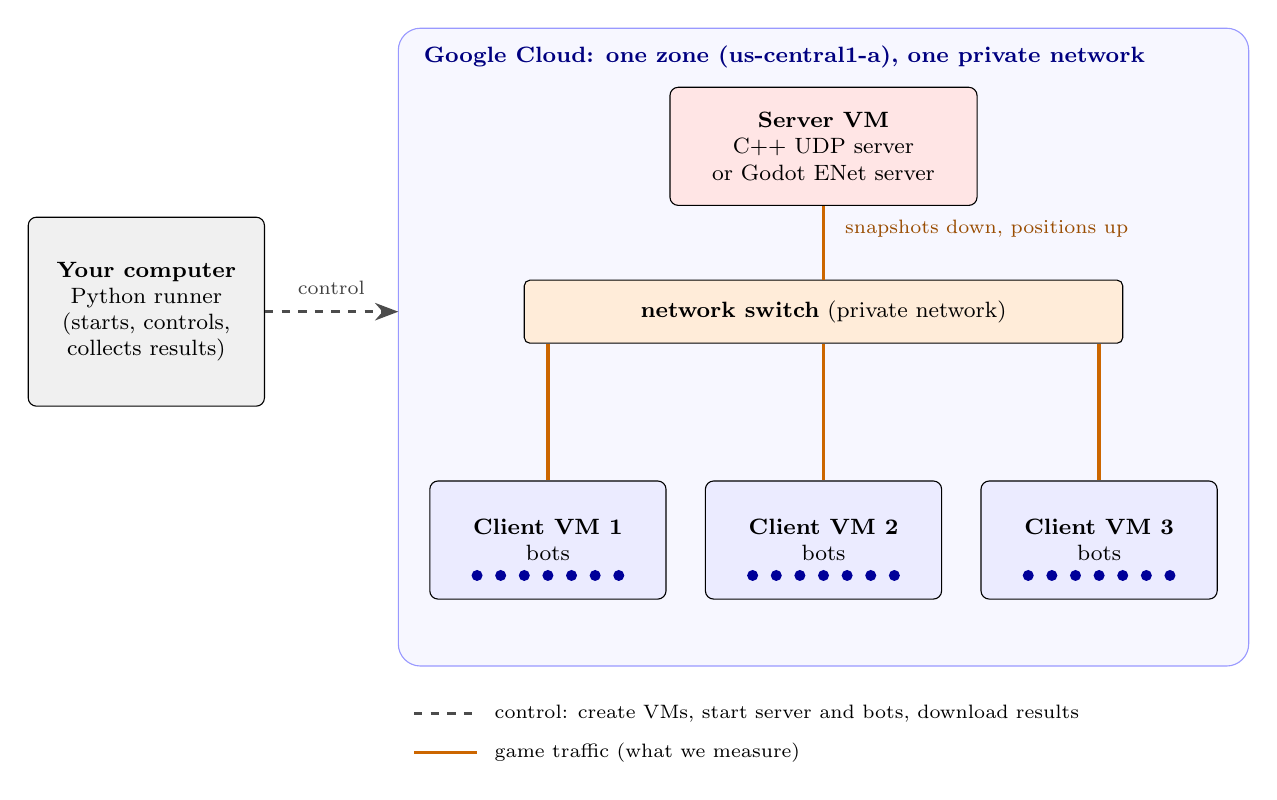
\begin{tikzpicture}[x=1cm,y=1cm,font=\footnotesize,
  vm/.style={draw,rounded corners=3pt,fill=blue!8,minimum width=3.0cm,minimum height=1.5cm,align=center,inner sep=4pt},
  srv/.style={draw,rounded corners=3pt,fill=red!10,minimum width=3.9cm,minimum height=1.5cm,align=center,inner sep=4pt},
  net/.style={orange!80!black,very thick}]
% cloud
\draw[rounded corners=8pt,fill=blue!3,draw=blue!40] (4.7,-4.6) rectangle (15.5,3.5);
\node[anchor=north west,font=\bfseries\footnotesize,text=blue!50!black] at (4.9,3.4) {Google Cloud: one zone (us-central1-a), one private network};
% runner
\node[draw,rounded corners=3pt,fill=gray!12,minimum width=3.0cm,minimum height=2.4cm,align=center] (run) at (1.5,-0.1) {\textbf{Your computer}\\ Python runner\\ (starts, controls,\\ collects results)};
\draw[gray!60!black,dashed,very thick,-{Stealth}] (run.east) -- (4.7,-0.1);
\node[font=\scriptsize,gray!50!black,align=center,anchor=south] at (3.85,0.0) {control};
% switch
\node[draw,rounded corners=2pt,fill=orange!15,minimum width=7.6cm,minimum height=0.8cm,align=center] (sw) at (10.1,-0.1) {\textbf{network switch} (private network)};
% server
\node[srv] (srv) at (10.1,2.0) {\textbf{Server VM}\\ C++ UDP server\\ or Godot ENet server};
% clients
\node[vm] (c1) at (6.6,-3.0) {\textbf{Client VM 1}\\ bots};
\node[vm] (c2) at (10.1,-3.0) {\textbf{Client VM 2}\\ bots};
\node[vm] (c3) at (13.6,-3.0) {\textbf{Client VM 3}\\ bots};
\foreach \x in {6.6,10.1,13.6} {\foreach \d in {-0.9,-0.6,...,0.9} {\fill[blue!60!black] (\x+\d,-3.45) circle (0.07);}}
% game traffic
\draw[net] (srv.south) -- (srv.south |- sw.north);
\foreach \c in {c1,c2,c3} {\draw[net] (\c.north) -- (\c.north |- sw.south);}
\node[font=\scriptsize,orange!60!black,anchor=west] at (10.25,0.95) {snapshots down, positions up};
% legend
\draw[gray!60!black,dashed,very thick] (4.9,-5.2) -- (5.7,-5.2);
\node[anchor=west,font=\scriptsize] at (5.8,-5.2) {control: create VMs, start server and bots, download results};
\draw[net] (4.9,-5.7) -- (5.7,-5.7);
\node[anchor=west,font=\scriptsize] at (5.8,-5.7) {game traffic (what we measure)};
\end{tikzpicture}
\caption{Where a test runs. The runner on your computer creates one server VM and
three client VMs, starts the server, tells each client VM how many bots to run,
and downloads the results afterwards. The bots and the server talk to each other
over the cloud's private network (a switch). Each client VM runs about a third of
the bots, so the server sees all of them as one crowd.}
\label{fig:fleet}
\end{figure}

Gaps and incomplete snapshots are indicators of protocol-level loss, not
measured network packet-loss percentages.


\subsection{What the charts show}
Every chart plots the same four things for both backends:

\begin{itemize}
\item \textbf{Latency:} average ping.
\item \textbf{Packet handling:} snapshots received per client per second.
\item \textbf{Clients responding:} how many clients are still getting answers.
\item \textbf{Tick rate:} server ticks per second.
\end{itemize}

On the ladder charts the horizontal axis is the number of clients, so each point is one client count. On the hold charts it is time, so each point is one 10~s window.


\subsection{Health criteria and caveats}
TODO: write the pass/fail limits and what the measurements can and cannot show.

\subsection{Runs}

Granular ramps with $N_{\max}=300$ give 292 states per backend
($1$ plus $10$ through $300$).

\begin{table}[H]
\centering
\small
\begin{tabular}{@{}llllrrl@{}}
\toprule
Date (2026) & Type & Backend & Counts & Time/state & Runs & Status \\
\midrule
Oct 16--17 & Progressive ladder & C++, ENet & 1, 10--300 & 10~s & 8 runs & ok \\
Oct 17--19 & Hold & C++, ENet & 180, 260, 270, 300 & 20~min hold & 8 runs & ok \\
\bottomrule
\end{tabular}
\caption{Runs used in the results. The progressive ladder is eight complete runs per backend, each run a separate pass from 1 to 300 clients (one repetition each). Each hold target is also eight runs; the ENet captures that runs 3 and 4 were missing were repeated in a separate make-up batch.}
\end{table}


\section{Results}\label{sec:results}

\subsection{Test 1, progressive ladder: full run}
Figure~\ref{fig:ladder} is the progressive ladder test (Section~\ref{sec:data}). Clients are
added one at a time from 1 to 300, so each point is one client count. Each line is the mean of 8 complete runs, and the shaded band shows the lowest and highest run.

\begin{figure}[!htbp]
\centering
{\bfseries\small Test 1: progressive ladder, 1 to 300 clients, both backends (mean of 8 runs)\par}\vspace{4pt}
\begin{tikzpicture}
\begin{groupplot}[group style={group size=2 by 3,horizontal sep=1.7cm,vertical sep=1.9cm},
  width=0.5\textwidth,height=4.3cm,xlabel={clients},xmin=0,xmax=300,
  tick label style={font=\scriptsize},label style={font=\footnotesize},
  title style={font=\footnotesize\bfseries},grid=major,grid style={gray!25}]
\nextgroupplot[title={Latency (ping)},ylabel={ms},ymode=log]
\addplot[name path=pingca,draw=none,forget plot] table[col sep=comma,x=clients_target,y=ping_min]{data/final_cpp.csv};
\addplot[name path=pingcb,draw=none,forget plot] table[col sep=comma,x=clients_target,y=ping_max]{data/final_cpp.csv};
\addplot[blue!30,opacity=0.6,forget plot] fill between[of=pingca and pingcb];
\addplot[blue!70!black,thin,mark=*,mark size=0.4pt] table[col sep=comma,x=clients_target,y=ping_mean]{data/final_cpp.csv};
\addplot[name path=pingea,draw=none,forget plot] table[col sep=comma,x=clients_target,y=ping_min]{data/final_enet.csv};
\addplot[name path=pingeb,draw=none,forget plot] table[col sep=comma,x=clients_target,y=ping_max]{data/final_enet.csv};
\addplot[red!30,opacity=0.6,forget plot] fill between[of=pingea and pingeb];
\addplot[red!70!black,thin,mark=*,mark size=0.4pt] table[col sep=comma,x=clients_target,y=ping_mean]{data/final_enet.csv};
\nextgroupplot[title={Packet handling},ylabel={snapshots/s per client},ymin=0,ymax=38]
\addplot[name path=recvca,draw=none,forget plot] table[col sep=comma,x=clients_target,y=recv_min]{data/final_cpp.csv};
\addplot[name path=recvcb,draw=none,forget plot] table[col sep=comma,x=clients_target,y=recv_max]{data/final_cpp.csv};
\addplot[blue!30,opacity=0.6,forget plot] fill between[of=recvca and recvcb];
\addplot[blue!70!black,thin,mark=*,mark size=0.4pt] table[col sep=comma,x=clients_target,y=recv_mean]{data/final_cpp.csv};
\addplot[name path=recvea,draw=none,forget plot] table[col sep=comma,x=clients_target,y=recv_min]{data/final_enet.csv};
\addplot[name path=recveb,draw=none,forget plot] table[col sep=comma,x=clients_target,y=recv_max]{data/final_enet.csv};
\addplot[red!30,opacity=0.6,forget plot] fill between[of=recvea and recveb];
\addplot[red!70!black,thin,mark=*,mark size=0.4pt] table[col sep=comma,x=clients_target,y=recv_mean]{data/final_enet.csv};
\addplot[black,dashed,domain=0:300,samples=2]{20};
\nextgroupplot[title={Clients responding},ylabel={\%},ymin=80,ymax=101]
\addplot[name path=respca,draw=none,forget plot] table[col sep=comma,x=clients_target,y=resp_min]{data/final_cpp.csv};
\addplot[name path=respcb,draw=none,forget plot] table[col sep=comma,x=clients_target,y=resp_max]{data/final_cpp.csv};
\addplot[blue!30,opacity=0.6,forget plot] fill between[of=respca and respcb];
\addplot[blue!70!black,thin,mark=*,mark size=0.4pt] table[col sep=comma,x=clients_target,y=resp_mean]{data/final_cpp.csv};
\addplot[name path=respea,draw=none,forget plot] table[col sep=comma,x=clients_target,y=resp_min]{data/final_enet.csv};
\addplot[name path=respeb,draw=none,forget plot] table[col sep=comma,x=clients_target,y=resp_max]{data/final_enet.csv};
\addplot[red!30,opacity=0.6,forget plot] fill between[of=respea and respeb];
\addplot[red!70!black,thin,mark=*,mark size=0.4pt] table[col sep=comma,x=clients_target,y=resp_mean]{data/final_enet.csv};
\nextgroupplot[title={Server tick rate},ylabel={Hz},ymin=15,ymax=21]
\addplot[name path=tickca,draw=none,forget plot] table[col sep=comma,x=clients_target,y=tick_min]{data/final_cpp.csv};
\addplot[name path=tickcb,draw=none,forget plot] table[col sep=comma,x=clients_target,y=tick_max]{data/final_cpp.csv};
\addplot[blue!30,opacity=0.6,forget plot] fill between[of=tickca and tickcb];
\addplot[blue!70!black,thin,mark=*,mark size=0.4pt] table[col sep=comma,x=clients_target,y=tick_mean]{data/final_cpp.csv};
\addplot[name path=tickea,draw=none,forget plot] table[col sep=comma,x=clients_target,y=tick_min]{data/final_enet.csv};
\addplot[name path=tickeb,draw=none,forget plot] table[col sep=comma,x=clients_target,y=tick_max]{data/final_enet.csv};
\addplot[red!30,opacity=0.6,forget plot] fill between[of=tickea and tickeb];
\addplot[red!70!black,thin,mark=*,mark size=0.4pt] table[col sep=comma,x=clients_target,y=tick_mean]{data/final_enet.csv};
\addplot[black,dashed,domain=0:300,samples=2]{18};
\nextgroupplot[title={Server CPU use},ylabel={\% of the server VM},ymin=0,ymax=35]
\addplot[name path=scpuca,draw=none,forget plot] table[col sep=comma,x=clients_target,y=scpu_min]{data/final_cpp.csv};
\addplot[name path=scpucb,draw=none,forget plot] table[col sep=comma,x=clients_target,y=scpu_max]{data/final_cpp.csv};
\addplot[blue!30,opacity=0.6,forget plot] fill between[of=scpuca and scpucb];
\addplot[blue!70!black,thin,mark=*,mark size=0.4pt] table[col sep=comma,x=clients_target,y=scpu_mean]{data/final_cpp.csv};
\addplot[name path=scpuea,draw=none,forget plot] table[col sep=comma,x=clients_target,y=scpu_min]{data/final_enet.csv};
\addplot[name path=scpueb,draw=none,forget plot] table[col sep=comma,x=clients_target,y=scpu_max]{data/final_enet.csv};
\addplot[red!30,opacity=0.6,forget plot] fill between[of=scpuea and scpueb];
\addplot[red!70!black,thin,mark=*,mark size=0.4pt] table[col sep=comma,x=clients_target,y=scpu_mean]{data/final_enet.csv};
\end{groupplot}
\node[anchor=north] at (\linewidth/2-3.5cm,-12.5cm) {\footnotesize \textcolor{blue!70!black}{\rule[0.5ex]{1.2em}{1.2pt}} C++ UDP \quad \textcolor{red!70!black}{\rule[0.5ex]{1.2em}{1.2pt}} Godot ENet \quad shaded: lowest to highest run};
\end{tikzpicture}
\caption{Test 1, progressive ladder (16--17 October, 10~s per state). Each line is the mean of 8 complete runs and the shaded band spans the lowest to the highest run. Ping is on a log scale. Dashed lines: 20 snapshots per second (one per tick) and the 18~Hz threshold. Server CPU use is the mean over each state, read from the server VM. ENet values above 20 snapshots per second cannot be real, since the server ticks at 20~Hz; they appear to come from delayed log reads under heavy load.}
\label{fig:ladder}
\end{figure}

\paragraph{Why the C++ tick rate is below 20 Hz.} The C++ server checks the clock every few milliseconds and starts each tick a little after 50~ms have passed. Each tick is slightly late, so it completes about 19 ticks per second instead of 20. This is a small built-in delay, not overload, and the line stays above the 18~Hz threshold.

Figure~\ref{fig:drift} counts the ticks of both servers side by side, Figure~\ref{lst:tick} is the code behind it and Figure~\ref{lst:pseudo} explains it in pseudocode. The loop starts a tick as soon as it notices that 50~ms have passed, and then restarts its timer from that moment. If it notices 2~ms late, the next 50~ms are counted from the late moment, so the delay is never made up and each tick is 52~ms after the last. In 1~s that is $1000/52 \approx 19.2$ ticks instead of 20. In the measured data the tick rate falls from about 19.4~Hz (a 51.5~ms tick, about 1.5~ms late) with few clients to about 18.9~Hz (a 52.9~ms tick, about 2.9~ms late) at 300 clients, because with more clients each pass through the loop does more work, so the check for the next tick comes later.

\begin{figure}[H]
\centering
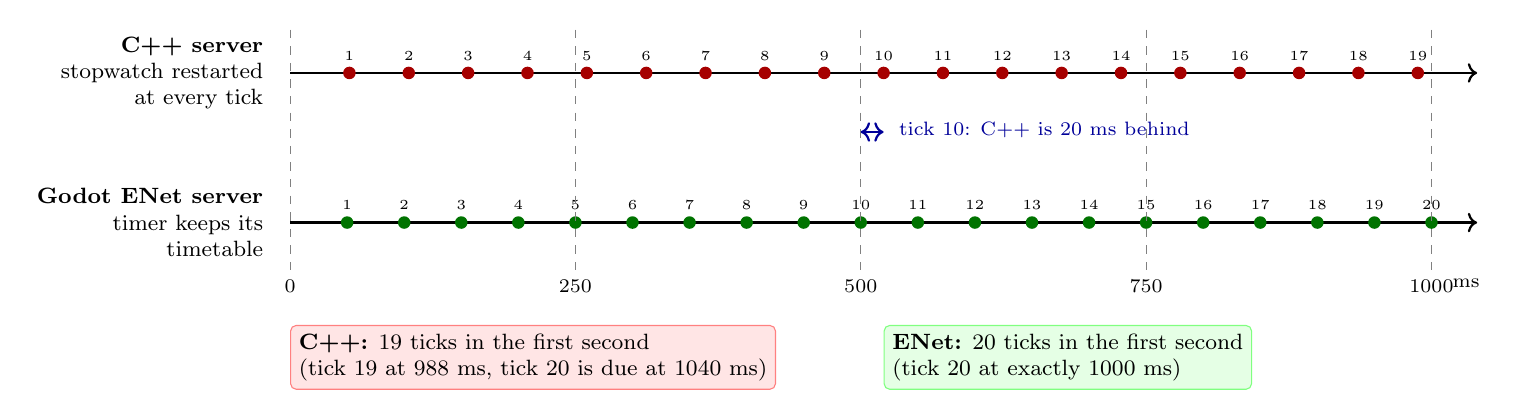
\begin{tikzpicture}[x=0.0145cm,y=1cm,font=\footnotesize,
  cpp/.style={circle,fill=red!65!black,inner sep=1.6pt},
  gd/.style={circle,fill=green!45!black,inner sep=1.6pt},
  num/.style={font=\tiny,inner sep=1pt}]
% one second timeline
\node[anchor=east,align=right] at (-15,0) {\textbf{C++ server}\\ stopwatch restarted\\ at every tick};
\node[anchor=east,align=right] at (-15,-1.9) {\textbf{Godot ENet server}\\ timer keeps its\\ timetable};
\draw[->,thick] (0,0) -- (1040,0);
\draw[->,thick] (0,-1.9) -- (1040,-1.9);
% C++ ticks every 52 ms (each tick noticed 2 ms late, delay never made up)
\foreach \k in {1,...,19} {\node[cpp] at (52*\k,0) {}; \node[num,anchor=south] at (52*\k,0.12) {\k};}
% ENet ticks every 50 ms
\foreach \k in {1,...,20} {\node[gd] at (50*\k,-1.9) {}; \node[num,anchor=south] at (50*\k,-1.78) {\k};}
% reference lines
\foreach \t in {0,250,500,750,1000} {\draw[gray,dashed] (\t,0.55) -- (\t,-2.5); \node[font=\scriptsize,anchor=north] at (\t,-2.5) {\t};}
\node[font=\scriptsize,anchor=north west] at (1010,-2.5) {ms};
% gap after 10 ticks
\draw[<->,thick,blue!60!black] (500,-0.75) -- (520,-0.75);
\node[font=\scriptsize,blue!60!black,anchor=south west] at (525,-0.95) {tick 10: C++ is 20 ms behind};
% totals
\node[anchor=north west,fill=red!10,draw=red!50,rounded corners=2pt,inner sep=3pt,align=left] at (0,-3.2) {\textbf{C++:} 19 ticks in the first second\\ (tick 19 at 988 ms, tick 20 is due at 1040 ms)};
\node[anchor=north west,fill=green!10,draw=green!50,rounded corners=2pt,inner sep=3pt,align=left] at (520,-3.2) {\textbf{ENet:} 20 ticks in the first second\\ (tick 20 at exactly 1000 ms)};
\end{tikzpicture}
\caption{Counting ticks, C++ against ENet (schematic, each tick noticed 2~ms late). Every dot is one tick and the number is the tick count. The C++ loop restarts its stopwatch at each tick, so its ticks are 52~ms apart and it has counted only 19 ticks after one second. The Godot timer keeps its 50~ms timetable, so its tick 20 arrives at exactly 1000~ms. After 10 ticks the C++ server is already 20~ms behind, and the gap keeps growing.}
\label{fig:drift}
\end{figure}

\begin{figure}[H]
\begin{lstlisting}[language=C++]
// current code (server/main.cpp): the tick loop
auto   now     = Clock::now();
double elapsed = std::chrono::duration<double>(now - last_tick).count();
if (elapsed >= TICK_SEC) {      // 50 ms or more have passed
    last_tick = now;            // restart the timer at "now": the delay is lost
    tick_n++;
    // ... drop silent clients, broadcast snapshots ...
}

// fix (not applied): advance the timer by exactly one tick
last_tick += std::chrono::duration_cast<Clock::duration>(
                 std::chrono::duration<double>(TICK_SEC));
\end{lstlisting}
\caption{The tick check in the C++ server and the one-line change that would remove the drift.}
\label{lst:tick}
\end{figure}

\begin{figure}[H]
\begin{lstlisting}[language={}]
STOPWATCH (the C++ server today)     TIMETABLE (Godot timer / the fix)
-------------------------------     ---------------------------------
every loop:                          every loop:
  if now - last_tick >= 50 ms:         if now - last_tick >= 50 ms:
    last_tick = now                      last_tick = last_tick + 50 ms
    do the tick                          do the tick

Stopwatch: noticed at 52 ms -> next tick due at 52 + 50 = 102 ms (drifts).
Timetable: noticed at 52 ms -> next tick due at 50 + 50 = 100 ms (on schedule).
\end{lstlisting}
\caption{Pseudocode for the two ways of timing a tick. Think of a bus that should leave every 50 minutes: the stopwatch driver restarts his watch whenever he notices the bus is due, so any lateness is kept; the timetable driver follows fixed times, so lateness is not kept.}
\label{lst:pseudo}
\end{figure}


\subsection{Test 2, hold at 300 clients: ramp-up and hold}
Figure~\ref{fig:hold300} is the hold test at 300 clients, the heaviest target, summed up over 8 runs. The grey left part is the ramp-up, when clients are being added (plus a short wait); time 0 is the moment the hold starts and no more clients are added. What matters is whether the lines recover after the ramp-up. C++ is steady in every run. ENet starts to fall behind during the ramp-up and does not recover: during the hold on average about 75\% of its clients respond (61 to 88\% across runs), it delivers about 16 snapshots per client per second, and its ping is around 1.4~s.

\begin{figure}[!htbp]
\centering
{\bfseries\small Test 2: hold at 300 clients, ramp-up then 20-minute hold (mean of 8 runs)\par}\vspace{4pt}
\begin{tikzpicture}
\begin{groupplot}[group style={group size=2 by 2,horizontal sep=1.7cm,vertical sep=2.2cm},
  width=0.5\textwidth,height=5cm,xlabel={minutes (0 = hold starts)},xmin=-8,xmax=20,
  tick label style={font=\scriptsize},label style={font=\footnotesize},
  title style={font=\footnotesize\bfseries},grid=major,grid style={gray!25}]
\nextgroupplot[title={Latency (ping)},ylabel={ms},ymin=2,ymax=6000,ymode=log]
\fill[gray!18] (axis cs:-8,2) rectangle (axis cs:0,6000);
\addplot[name path=pingca,draw=none,forget plot] table[col sep=comma,x=minute_rel,y=ping_min]{data/finalhold_cpp_300.csv};
\addplot[name path=pingcb,draw=none,forget plot] table[col sep=comma,x=minute_rel,y=ping_max]{data/finalhold_cpp_300.csv};
\addplot[blue!30,opacity=0.6,forget plot] fill between[of=pingca and pingcb];
\addplot[blue!70!black,thin,mark=*,mark size=0.4pt] table[col sep=comma,x=minute_rel,y=ping_mean]{data/finalhold_cpp_300.csv};
\addplot[name path=pingea,draw=none,forget plot] table[col sep=comma,x=minute_rel,y=ping_min]{data/finalhold_enet_300.csv};
\addplot[name path=pingeb,draw=none,forget plot] table[col sep=comma,x=minute_rel,y=ping_max]{data/finalhold_enet_300.csv};
\addplot[red!30,opacity=0.6,forget plot] fill between[of=pingea and pingeb];
\addplot[red!70!black,thin,mark=*,mark size=0.4pt] table[col sep=comma,x=minute_rel,y=ping_mean]{data/finalhold_enet_300.csv};
\nextgroupplot[title={Packet handling},ylabel={snapshots/s per client},ymin=0,ymax=24]
\fill[gray!18] (axis cs:-8,0) rectangle (axis cs:0,24);
\addplot[name path=recvca,draw=none,forget plot] table[col sep=comma,x=minute_rel,y=recv_min]{data/finalhold_cpp_300.csv};
\addplot[name path=recvcb,draw=none,forget plot] table[col sep=comma,x=minute_rel,y=recv_max]{data/finalhold_cpp_300.csv};
\addplot[blue!30,opacity=0.6,forget plot] fill between[of=recvca and recvcb];
\addplot[blue!70!black,thin,mark=*,mark size=0.4pt] table[col sep=comma,x=minute_rel,y=recv_mean]{data/finalhold_cpp_300.csv};
\addplot[name path=recvea,draw=none,forget plot] table[col sep=comma,x=minute_rel,y=recv_min]{data/finalhold_enet_300.csv};
\addplot[name path=recveb,draw=none,forget plot] table[col sep=comma,x=minute_rel,y=recv_max]{data/finalhold_enet_300.csv};
\addplot[red!30,opacity=0.6,forget plot] fill between[of=recvea and recveb];
\addplot[red!70!black,thin,mark=*,mark size=0.4pt] table[col sep=comma,x=minute_rel,y=recv_mean]{data/finalhold_enet_300.csv};
\addplot[black,dashed,domain=-8:20,samples=2]{20};
\nextgroupplot[title={Clients responding},ylabel={\% of connected},ymin=0,ymax=105]
\fill[gray!18] (axis cs:-8,0) rectangle (axis cs:0,105);
\addplot[name path=responding_pctca,draw=none,forget plot] table[col sep=comma,x=minute_rel,y=responding_pct_min]{data/finalhold_cpp_300.csv};
\addplot[name path=responding_pctcb,draw=none,forget plot] table[col sep=comma,x=minute_rel,y=responding_pct_max]{data/finalhold_cpp_300.csv};
\addplot[blue!30,opacity=0.6,forget plot] fill between[of=responding_pctca and responding_pctcb];
\addplot[blue!70!black,thin,mark=*,mark size=0.4pt] table[col sep=comma,x=minute_rel,y=responding_pct_mean]{data/finalhold_cpp_300.csv};
\addplot[name path=responding_pctea,draw=none,forget plot] table[col sep=comma,x=minute_rel,y=responding_pct_min]{data/finalhold_enet_300.csv};
\addplot[name path=responding_pcteb,draw=none,forget plot] table[col sep=comma,x=minute_rel,y=responding_pct_max]{data/finalhold_enet_300.csv};
\addplot[red!30,opacity=0.6,forget plot] fill between[of=responding_pctea and responding_pcteb];
\addplot[red!70!black,thin,mark=*,mark size=0.4pt] table[col sep=comma,x=minute_rel,y=responding_pct_mean]{data/finalhold_enet_300.csv};
\nextgroupplot[title={Server tick rate},ylabel={Hz},ymin=15,ymax=21]
\fill[gray!18] (axis cs:-8,15) rectangle (axis cs:0,21);
\addplot[name path=tickca,draw=none,forget plot] table[col sep=comma,x=minute_rel,y=tick_min]{data/finalhold_cpp_300.csv};
\addplot[name path=tickcb,draw=none,forget plot] table[col sep=comma,x=minute_rel,y=tick_max]{data/finalhold_cpp_300.csv};
\addplot[blue!30,opacity=0.6,forget plot] fill between[of=tickca and tickcb];
\addplot[blue!70!black,thin,mark=*,mark size=0.4pt] table[col sep=comma,x=minute_rel,y=tick_mean]{data/finalhold_cpp_300.csv};
\addplot[name path=tickea,draw=none,forget plot] table[col sep=comma,x=minute_rel,y=tick_min]{data/finalhold_enet_300.csv};
\addplot[name path=tickeb,draw=none,forget plot] table[col sep=comma,x=minute_rel,y=tick_max]{data/finalhold_enet_300.csv};
\addplot[red!30,opacity=0.6,forget plot] fill between[of=tickea and tickeb];
\addplot[red!70!black,thin,mark=*,mark size=0.4pt] table[col sep=comma,x=minute_rel,y=tick_mean]{data/finalhold_enet_300.csv};
\addplot[black,dashed,domain=-8:20,samples=2]{18};
\end{groupplot}
\node[anchor=north] at (\linewidth/2-3.5cm,-9.0cm) {\footnotesize \textcolor{blue!70!black}{\rule[0.5ex]{1.2em}{1.2pt}} C++ UDP \quad \textcolor{red!70!black}{\rule[0.5ex]{1.2em}{1.2pt}} Godot ENet \quad shaded band: lowest to highest run};
\end{tikzpicture}
\caption{Test 2, hold at 300 clients, one point per 10~s. Each line is the mean of 8 runs and the band spans the lowest to the highest run. Grey: clients being added (ramp-up and a short wait before the hold). White: the 20-minute hold. Dashed lines: 20 snapshots per second and the 18~Hz threshold. ENet latency is the game client's logged ping; C++ latency is a raw round trip, so the two are not directly comparable (see Section~\ref{sec:data}).}
\label{fig:hold300}
\end{figure}

\subsection{Test 2, hold at every target}
Figure~\ref{fig:holdall} repeats the hold test for all four targets, again with the ramp-up on the left, and Table~\ref{tab:holdsum} sums up each target. C++ held every target in all eight runs. ENet held 180 clients in all eight runs, but only one of eight runs at 260 clients and one of eight at 270, and none at 300.

\begin{figure}[!htbp]
\centering
{\bfseries\small Test 2: hold test at every target, share of clients responding (mean of 8 runs)\par}\vspace{4pt}
\begin{tikzpicture}
\begin{groupplot}[group style={group size=2 by 2,horizontal sep=1.7cm,vertical sep=1.9cm},
  width=0.5\textwidth,height=4.3cm,xlabel={minutes (0 = hold starts)},xmin=-8,xmax=20,
  ymin=0,ymax=105,ylabel={\% responding},
  tick label style={font=\scriptsize},label style={font=\footnotesize},
  title style={font=\footnotesize\bfseries},grid=major,grid style={gray!25},
  legend style={font=\tiny,at={(1.02,0.5)},anchor=west}]
\nextgroupplot[title={C++ UDP, all four targets}]
\fill[gray!18] (axis cs:-8,0) rectangle (axis cs:0,105);
\addplot[red!70!black,thin,mark=none] table[col sep=comma,x=minute_rel,y=responding_pct_mean]{data/finalhold_cpp_180.csv};
\addplot[blue!70!black,thin,mark=none] table[col sep=comma,x=minute_rel,y=responding_pct_mean]{data/finalhold_cpp_260.csv};
\addplot[green!50!black,thin,mark=none] table[col sep=comma,x=minute_rel,y=responding_pct_mean]{data/finalhold_cpp_270.csv};
\addplot[orange!85!black,thin,mark=none] table[col sep=comma,x=minute_rel,y=responding_pct_mean]{data/finalhold_cpp_300.csv};
\nextgroupplot[title={Godot ENet, 260 clients}]
\fill[gray!18] (axis cs:-8,0) rectangle (axis cs:0,105);
\addplot[name path=e260a,draw=none,forget plot] table[col sep=comma,x=minute_rel,y=responding_pct_min]{data/finalhold_enet_260.csv};
\addplot[name path=e260b,draw=none,forget plot] table[col sep=comma,x=minute_rel,y=responding_pct_max]{data/finalhold_enet_260.csv};
\addplot[red!30,opacity=0.6,forget plot] fill between[of=e260a and e260b];
\addplot[red!70!black,thin,mark=none] table[col sep=comma,x=minute_rel,y=responding_pct_mean]{data/finalhold_enet_260.csv};
\nextgroupplot[title={Godot ENet, 270 clients}]
\fill[gray!18] (axis cs:-8,0) rectangle (axis cs:0,105);
\addplot[name path=e270a,draw=none,forget plot] table[col sep=comma,x=minute_rel,y=responding_pct_min]{data/finalhold_enet_270.csv};
\addplot[name path=e270b,draw=none,forget plot] table[col sep=comma,x=minute_rel,y=responding_pct_max]{data/finalhold_enet_270.csv};
\addplot[red!30,opacity=0.6,forget plot] fill between[of=e270a and e270b];
\addplot[red!70!black,thin,mark=none] table[col sep=comma,x=minute_rel,y=responding_pct_mean]{data/finalhold_enet_270.csv};
\nextgroupplot[title={Godot ENet, 300 clients}]
\fill[gray!18] (axis cs:-8,0) rectangle (axis cs:0,105);
\addplot[name path=e300a,draw=none,forget plot] table[col sep=comma,x=minute_rel,y=responding_pct_min]{data/finalhold_enet_300.csv};
\addplot[name path=e300b,draw=none,forget plot] table[col sep=comma,x=minute_rel,y=responding_pct_max]{data/finalhold_enet_300.csv};
\addplot[red!30,opacity=0.6,forget plot] fill between[of=e300a and e300b];
\addplot[red!70!black,thin,mark=none] table[col sep=comma,x=minute_rel,y=responding_pct_mean]{data/finalhold_enet_300.csv};
\end{groupplot}
\end{tikzpicture}
\caption{Test 2, share of clients responding during the hold at every target (mean of 8 runs). Grey: ramp-up. Top left: C++ UDP at 180, 260, 270 and 300 clients stays at 100\% (all four lines overlap). The other panels show Godot ENet at 260, 270 and 300 clients; the line is the mean of 8 runs and the red band spans the lowest to the highest run. ENet at 180 clients also stays at 100\% in all 8 runs and is not shown.}
\label{fig:holdall}
\end{figure}

\begin{table}[H]
\centering
\small
\setlength{\tabcolsep}{4pt}
\begin{tabular}{@{}lrrrrrl@{}}
\toprule
Backend & Clients & Resp. (\%) & Snap/s & Ping, ms & Tick (Hz) & Held \\
\midrule
C++ UDP & 180 & 100.0 (100.0--100.0) & 19.0 & 5 (5--6) & 19.0 & 8 of 8 \\
C++ UDP & 260 & 100.0 (100.0--100.0) & 18.8 & 6 (6--6) & 18.8 & 8 of 8 \\
C++ UDP & 270 & 100.0 (100.0--100.0) & 18.8 & 6 (6--6) & 18.8 & 8 of 8 \\
C++ UDP & 300 & 100.0 (100.0--100.0) & 18.8 & 6 (6--6) & 18.8 & 8 of 8 \\
\midrule
Godot ENet & 180 & 100.0 (100.0--100.0) & 20.0 & 36 (35--36) & 20.0 & 8 of 8 \\
Godot ENet & 260 & 93.2 (87.8--100.0) & 19.3 & 701 (106--1267) & 20.0 & 1 of 8 \\
Godot ENet & 270 & 86.9 (76.7--100.0) & 18.5 & 927 (113--1612) & 20.0 & 1 of 8 \\
Godot ENet & 300 & 75.2 (61.1--88.4) & 15.9 & 1356 (924--1908) & 20.0 & 0 of 8 \\
\bottomrule
\end{tabular}
\caption{Hold results at each target, summed up over 8 runs. Each run is first averaged over its 20-minute hold; the table gives the mean of those averages with the lowest and highest run in brackets. Resp. = clients responding, Snap/s = snapshots received per client per second, Tick = server ticks per second. A run ``held'' if its hold averages met the health limits (at least 99\% responding, at least 18 snapshots per second, ping at most 150~ms, tick at least 18~Hz). C++ ping is a raw round trip and ENet ping is the game client's ping, so they are not directly comparable.}
\label{tab:holdsum}
\end{table}

\subsection{Example data}
The tables below are real rows from our runs, to show what the data looks like.

\paragraph{Progressive ladder: 8 runs summed up.}
Each row sums up the 8 complete ladder runs at one client count: the mean, with the lowest and highest run in brackets. Resp. = clients responding (mean), Snap/s = snapshots received per client per second, Tick = server ticks per second, Passing = runs that met the health limits at that count.

\begin{table}[H]
\centering
\small
\setlength{\tabcolsep}{4pt}
\begin{tabular}{@{}lrrrrrl@{}}
\toprule
Backend & Clients & Resp. (\%) & Ping, ms & Snap/s & Tick (Hz) & Passing \\
\midrule
C++ UDP & 100 & 100.0 & 5 (5--5) & 19.1 (19.1--19.3) & 19.1 & 8 of 8 \\
C++ UDP & 150 & 100.0 & 5 (5--5) & 19.1 (19.0--19.2) & 19.1 & 8 of 8 \\
C++ UDP & 200 & 100.0 & 5 (5--6) & 19.0 (18.8--19.1) & 19.0 & 8 of 8 \\
C++ UDP & 250 & 100.0 & 6 (5--6) & 18.9 (18.8--19.1) & 18.9 & 8 of 8 \\
C++ UDP & 300 & 100.0 & 6 (6--6) & 18.9 (18.8--19.0) & 19.3 & 8 of 8 \\
\midrule
Godot ENet & 100 & 100.0 & 29 (28--31) & 19.9 (19.8--19.9) & 20.0 & 8 of 8 \\
Godot ENet & 150 & 100.0 & 33 (31--34) & 19.6 (19.3--19.9) & 20.0 & 8 of 8 \\
Godot ENet & 200 & 100.0 & 38 (34--42) & 18.0 (16.5--20.2) & 20.0 & 3 of 8 \\
Godot ENet & 250 & 100.0 & 478 (46--942) & 14.4 (12.8--17.6) & 20.0 & 0 of 8 \\
Godot ENet & 300 & 99.3 & 252 (50--1474) & 31.2 (28.2--35.8) & 20.0 & 3 of 8 \\
\bottomrule
\end{tabular}
\caption{Example ladder rows, summed up over 8 runs (16--17 October, 10~s per state). Ping and Snap/s show the mean and, in brackets, the lowest and highest run. C++ ping is a raw round trip and ENet ping is the game client's ping, so they are not directly comparable.}
\end{table}

\noindent\textbf{Two things to note.}
First, the two backends measure latency differently: for C++ it is a raw round
trip from a dedicated ping message, while for ENet it is the game client's
logged ping (time until the next snapshot). They are not directly comparable
until the Method section states how each is handled. Second, the ENet server's
tick rate stays near 20~Hz even when its clients are failing, so for ENet the
breakdown shows up as lost clients, low snapshot rate and high ping rather than
a tick-rate drop. TODO: confirm why. The ENet server counts ticks from a Godot timer that fires every 50~ms without drift, so its tick counter keeps pace with the clock whether or not the work finished in time.

\subsection{How the runs were summed up}
Both tests combine 8 complete runs per backend. For the ladder, each of the 292 client counts is paired with the same count in the other runs. For the holds, each 10~s state is paired by its position in the ramp-up or hold. The mean, lowest and highest value of each measure are reported. A ladder run passes at a client count if that count met the health limits; a hold run held if its hold averages met them. Hold runs 3 and 4 were missing some ENet captures because those captures failed, so they were repeated in a separate make-up batch and used in their place (ENet 270 and 300 clients for run 3, ENet 300 clients for run 4).

\section{Discussion}
TODO.

\section{Conclusion}
TODO.

\begin{thebibliography}{9}
\bibitem{aukstakalnis2024} L. Aukstakalnis. \emph{Server-Client Networking Implementation Using the Godot Game Engine}. 2024.
\bibitem{aldhief2018} F. T. Al-Dhief et al. Performance comparison between TCP and UDP protocols in different simulation
scenarios. \emph{International Journal of Engineering \& Technology}, 7(4.36):172--176, 2018.
\bibitem{jones2025} C. Jones. Go UDP programming: a beginner-friendly guide to building fast, real-time apps. DEV Community, 2025.
\bibitem{retunsky2023} E. Retunsky. Benchmarking low-level I/O: C, C++, Rust, Golang, Java, Python. Star Gazers, 2023.
\bibitem{godotdedicated} Godot Foundation. Exporting for dedicated servers. \emph{Godot Engine Documentation}, 2026.
\bibitem{godotudp} Godot Foundation. UDPServer. \emph{Godot Engine Documentation}, 2026.
\bibitem{unityticks} Unity Technologies. Ticks and update rates. \emph{Netcode for GameObjects 2.5 manual}.
\url{https://docs.unity3d.com/Packages/com.unity.netcode.gameobjects@2.5/manual/learn/ticks-and-update-rates.html}
\bibitem{valvesource} Valve Developer Community. Source Multiplayer Networking.
\url{https://developer.valvesoftware.com/wiki/Source_Multiplayer_Networking}
\end{thebibliography}

\end{document}
